\documentclass[border=3mm]{standalone}

\usepackage{pgfplots}

% Unit circle plot style
\pgfplotsset{unit circle/.style={width=4cm,height=4cm,axis lines=middle,xtick=\empty,ytick=\empty,axis equal,enlargelimits,xmax=1,ymax=1,xmin=-1,ymin=-1,domain=0:pi/2}}

\renewcommand{\familydefault}{\sfdefault}
\pgfplotsset{compat=1.10}

\usepgfplotslibrary{fillbetween}

\begin{document}
    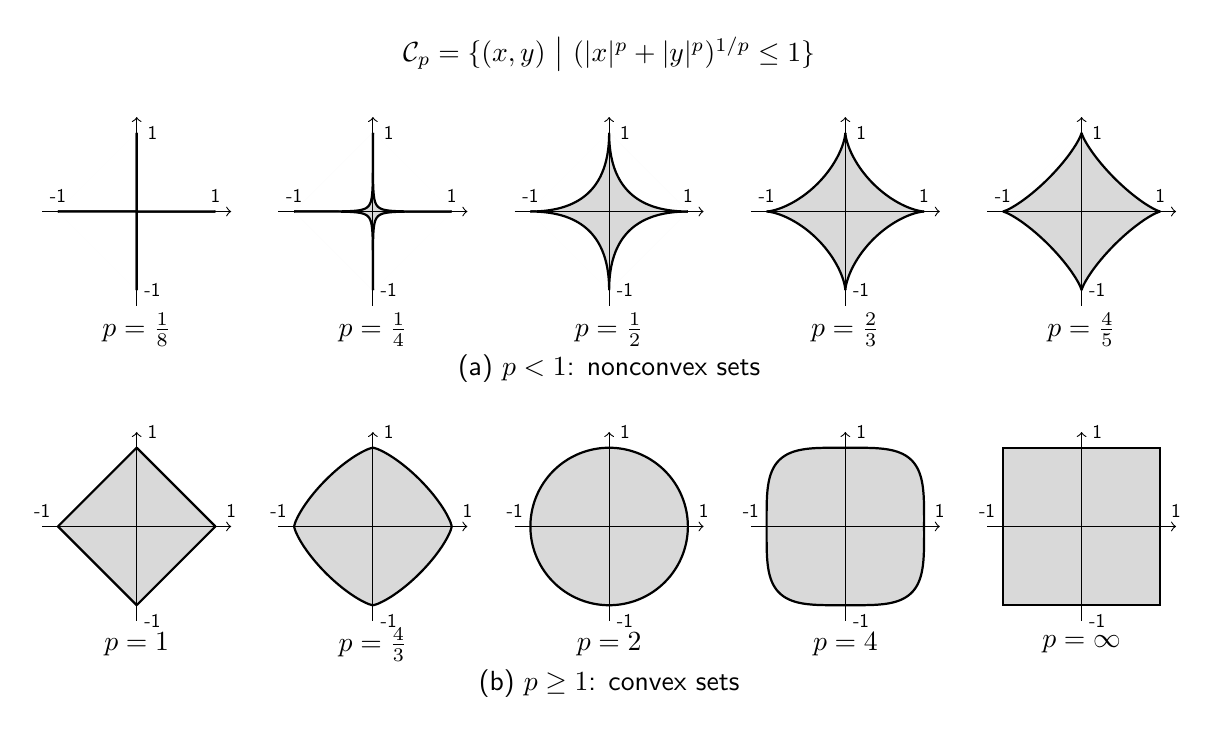
\begin{tikzpicture}
    
    \def\d{3}
    \foreach \t/\p in {0/16, 1/8, 2/4, 3/3, 4/2.5} {
    \begin{scope}[xshift = \t*\d cm]        
       % \def\p{16}
        \draw [fill = gray!30, draw = white] (1, 0)  --  (0, 1)  --  (-1, 0)  --  (0, -1)  --  cycle;
        \draw[black, thick, fill = white, scale=1,domain=0:90,samples=100,smooth,variable=\t]
          plot({-1*cos(\t)^(\p)},{1*sin(\t)^(\p)});
        \draw[black, thick,fill = white, scale=1,domain=0:90,samples=100,smooth,variable=\t]
          plot({-1*cos(\t)^(\p)},{-1*sin(\t)^(\p)});
        \draw[black, thick,fill = white, scale=1,domain=0:90,samples=100,smooth,variable=\t]
          plot({1*cos(\t)^(\p)},{-1*sin(\t)^(\p)});
        \draw[black, thick,fill = white, scale=1,domain=0:90,samples=100,smooth,variable=\t]
          plot({1*cos(\t)^(\p)},{1*sin(\t)^(\p)});                 

        \draw [->] (-1.2,0) -- (1.2,0);
        \draw [->] (0, -1.2) -- (0,1.2);
        \node [scale = .7] at (-1, .2) {-1};
        \node [scale = .7] at (1, .2) {1};
        \node [scale = .7] at (.2, 1) {1};
        \node [scale = .7] at (.2, -1) {-1};
    \end{scope}
    }

    \node at (0, -1.5) {$p = \frac{1}{8}$};
    \node at (\d, -1.5) {$p = \frac{1}{4}$};
    \node at (2*\d, -1.5) {$p = \frac{1}{2}$};
    \node at (3*\d, -1.5) {$p = \frac{2}{3}$};
    \node at (4*\d, -1.5) {$p = \frac{4}{5}$};

    \foreach \t/\p in {0/2, 1/1.5, 2/1, 3/.5} {
    \begin{scope}[xshift = \t*\d cm, yshift = -4cm]        
       % \def\p{16}
        \draw [fill = gray!30, draw = gray!30] (1, 0)  --  (0, 1)  --  (-1, 0)  --  (0, -1)  --  cycle;
        \draw[black, thick, fill = gray!30, scale=1,domain=0:90,samples=100,smooth,variable=\t]
          plot({-1*cos(\t)^(\p)},{1*sin(\t)^(\p)});
        \draw[black, thick,fill = gray!30, scale=1,domain=0:90,samples=100,smooth,variable=\t]
          plot({-1*cos(\t)^(\p)},{-1*sin(\t)^(\p)});
        \draw[black, thick,fill = gray!30, scale=1,domain=0:90,samples=100,smooth,variable=\t]
          plot({1*cos(\t)^(\p)},{-1*sin(\t)^(\p)});
        \draw[black, thick,fill = gray!30, scale=1,domain=0:90,samples=100,smooth,variable=\t]
          plot({1*cos(\t)^(\p)},{1*sin(\t)^(\p)});                 

        \draw [->] (-1.2,0) -- (1.2,0);
        \draw [->] (0, -1.2) -- (0,1.2);
        \node [scale = .7] at (-1.2, .2) {-1};
        \node [scale = .7] at (1.2, .2) {1};
        \node [scale = .7] at (.2, 1.2) {1};
        \node [scale = .7] at (.2, -1.2) {-1};
    \end{scope}
    }

     \begin{scope}[yshift = -4cm, xshift = 4*\d cm]
        \draw [black, thick, fill = gray!30] (-1, 1)  --  (1, 1)  --  (1, -1)  --  (-1, -1)  -- cycle;

         \draw [->] (-1.2,0) -- (1.2,0);
         \draw [->] (0, -1.2) -- (0,1.2);
         \node [scale = .7] at (-1.2, .2) {-1};
         \node [scale = .7] at (1.2, .2) {1};
         \node [scale = .7] at (.2, 1.2) {1};
         \node [scale = .7] at (.2, -1.2) {-1};
    \end{scope}

    \node at (0, -5.5) {$p = 1$};
    \node at (\d, -5.5) {$p = \frac{4}{3}$};
    \node at (2*\d, -5.5) {$p = 2$};
    \node at (3*\d, -5.5) {$p = 4$};
    \node at (4*\d, -5.5) {$p = \infty$};


    \node at (2*\d, 2) {$\mathcal{C}_p = \{(x, y)  ~\big| ~ (|x|^p + |y|^p)^{1/p} \leq 1\}$};

    \node at (2*\d, -2) {(a) $p < 1$: nonconvex sets};
    \node at (2*\d, -6) {(b) $p \geq 1$: convex sets};
    % \node at (-3, 0) {$p < 1$};
    % \node at (-3, -.5) {nonconvex sets};
    % \node at (-3, -4) {$p \geq 1$};
    % \node at (-3, -4.5) {convex sets};


\end{tikzpicture}
\end{document}